\documentclass[conference]{IEEEtran}
\usepackage{tikz}
\usetikzlibrary{positioning, arrows.meta, fit, calc}
\usepackage{amsmath}
\usepackage{amssymb}
\usepackage{listings}
\usepackage{xcolor}
\usepackage{booktabs}

\lstset{basicstyle=\ttfamily\scriptsize, breaklines=true, frame=single, framerule=0.2pt, backgroundcolor=\color{gray!5}}

\tikzset{
  block/.style={draw, rounded corners=2pt, minimum height=2.2em, minimum width=6em, align=center, font=\scriptsize},
  artifact/.style={block, fill=blue!8},
  process/.style={block, fill=orange!12},
  model/.style={block, fill=green!10},
  human/.style={block, fill=red!10},
  arr/.style={-{Stealth[length=2mm]}, thick},
  darr/.style={arr, dashed},
  lbl/.style={font=\tiny, midway}
}

\title{A Recipe-Based Model-Management Architecture for Versioned, Reproducible Training}

\author{
\IEEEauthorblockN{Johnny~Morgan}
\IEEEauthorblockA{Information Systems, UMBC\\
yj07538@umbc.edu}
}

\begin{document}
\maketitle

\begin{abstract}
We present a model-management architecture in which every trained model is reproducible because every input to its training is a versioned, re-executable artifact. Data acquisition is expressed as \emph{recipes}---recorded queries with time windows, snapshot dates, and join specifications against typed data sources (metadata, content, requirements). Labels are produced by versioned \emph{label rules} derived from a deterministic requirements repository, with human adjudications layered as versioned \emph{correction overlays} that never mutate the system of record. Models---trunks, classification heads, and baselines---are filesystem artifacts registered in a database with model cards, storage locations, hyperparameters, metrics, and a parent-model reference that makes fine-tuning lineage a directed acyclic graph. Orchestrated retraining at defined cadences (monthly head refresh, annual trunk fine-tuning) executes as recorded jobs, so reproducibility is a property of the system---re-execute the recipe---rather than a discipline asked of its operators. The architecture governs the frozen-trunk multi-customer classifier described in a companion paper~[1] and generalizes to any model program requiring auditable, versioned training.
\end{abstract}

\section{Introduction}
Model programs fail reproducibility not at training time but at data time: the model file survives while the query that built its training set, the requirements version that labeled it, and the corrections humans applied are lost. This architecture makes those inputs first-class artifacts. The organizing principle:

\begin{quote}
\emph{Reproducibility means the recipe re-executes---not that someone kept a copy of the dataframe.}
\end{quote}

Two storage roles divide cleanly: the \textbf{filesystem} holds every large artifact (datasets, embedding caches, model weights, model cards); the \textbf{database} is the spine---it holds identity, versions, locations, parameters, and every relationship between artifacts. Nothing is known to the platform unless it is a row; nothing heavy lives in a row.

\section{Data Source Abstraction}
Sources are typed by role, not by technology:
\begin{itemize}
\item \textbf{Metadata source (A):} defines populations and supplies join keys; pulls are windowed in time.
\item \textbf{Content source (B):} supplies the payload a model consumes (text here), joined by key.
\item \textbf{Requirements source (C):} the label authority; deterministic rules over C produce labels.
\end{itemize}
The typing is what generalizes: any program with a population source, a payload source, and a labeling authority maps onto the same schema.

\section{Recipes, Label Rules, and Correction Overlays}
Fig.~\ref{fig:flow} shows acquisition. A \textbf{dataset recipe} records the A query, time window, snapshot date, and B join specification; executing it materializes a dataset whose storage path and corpus hash are registered. A \textbf{label rule} records the C requirements reference and version per customer plus a rule hash; applying it to a dataset yields a \textbf{label set}, versioned and registered with class balance. Human adjudications (from the companion system's disagreement queue~[1]) are written to a \textbf{correction overlay}---a versioned table of per-record label amendments with adjudicator, timestamp, and the model version that surfaced the record. C is never mutated; the effective label is (label set $\oplus$ overlay), and every training job records which overlay version it consumed.

\begin{figure}[t]
\centering
\resizebox{\columnwidth}{!}{%
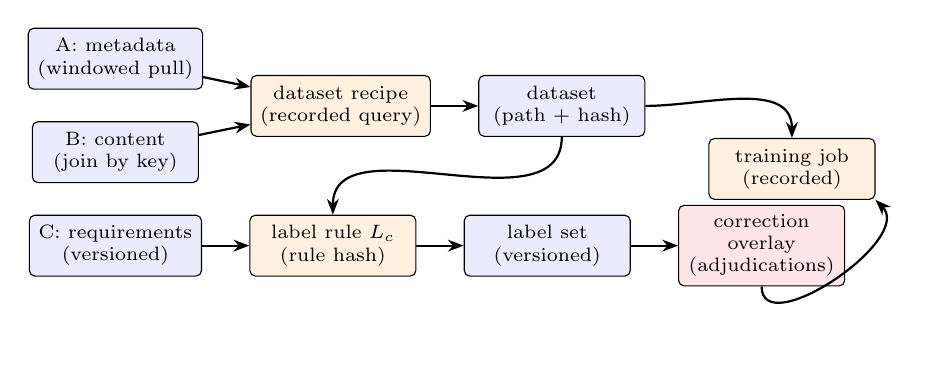
\begin{tikzpicture}[node distance=4mm and 6mm]
\node[artifact] (a) {A: metadata\\(windowed pull)};
\node[artifact, below=of a] (b) {B: content\\(join by key)};
\node[process, right=of a, yshift=-6mm] (rec) {dataset recipe\\(recorded query)};
\node[artifact, right=of rec] (ds) {dataset\\(path + hash)};
\node[artifact, below=of b] (c) {C: requirements\\(versioned)};
\node[process, right=of c] (lr) {label rule $L_c$\\(rule hash)};
\node[artifact, right=of lr] (ls) {label set\\(versioned)};
\node[human, right=of ls] (ov) {correction\\overlay\\(adjudications)};
\node[process, right=8mm of ds, yshift=-8mm] (train) {training job\\(recorded)};
\draw[arr] (a) -- (rec);
\draw[arr] (b) -- (rec);
\draw[arr] (rec) -- (ds);
\draw[arr] (c) -- (lr);
\draw[arr] (ds.south) to[out=-90,in=90] (lr.north);
\draw[arr] (lr) -- (ls);
\draw[arr] (ls) -- (ov);
\draw[arr] (ds.east) to[out=0,in=90] (train.north);
\draw[arr] (ov.south) to[out=-90,in=-45] (train.south east);
\end{tikzpicture}%
}
\caption{Acquisition as versioned artifacts: recipes materialize datasets; label rules over C produce label sets; adjudications overlay without mutating the system of record; training jobs record exactly which versions they consumed.}
\label{fig:flow}
\end{figure}

\section{Registry Schema}
\begin{lstlisting}
data_sources(id, name, role[A|B|C], connection_ref)
dataset_recipes(id, a_query, time_window,
    snapshot_date, b_join_spec, created_at)
datasets(id, recipe_id, storage_path,
    n_records, corpus_hash)
label_rules(id, customer_id, c_requirements_ref,
    requirements_version, rule_hash)
label_sets(id, dataset_id, label_rule_id,
    version, storage_path, class_balance)
correction_overlays(id, label_set_id, version,
    storage_path)
corrections(overlay_id, record_id, old_label,
    new_label, adjudicator, source_model_id, at)
feature_sets(id, version, extraction_spec,
    storage_path)
models(id, kind[trunk|head|baseline], name,
    version, parent_model_id, dataset_id,
    label_set_id, overlay_version,
    feature_set_id, trunk_model_id,
    storage_path, model_card_path,
    hyperparams_json, metrics_json,
    threshold, trained_at)
training_jobs(id, model_id, cadence
    [monthly|annual|on_demand], recipe_id,
    status, started_at, finished_at, log_path)
manifest(deployed_at, trunk_model_id,
    head_model_ids_json, committed_by)
\end{lstlisting}
Every column that names an artifact stores a filesystem path; every relationship is a foreign key. The model card is a human-readable file (scope, intended use, data description, metrics, caveats) whose location---not content---lives in the row.

\section{Model Lineage}
\texttt{parent\_model\_id} makes model history a DAG (Fig.~\ref{fig:dag}): a trunk fine-tuned from its predecessor, heads warm-started from prior heads, all heads referencing the trunk (and feature-set version) they consume. Lineage answers the audit question in one query: for any deployed prediction, which head version, trained on which dataset and label versions including which adjudications, descended from which parents, against which trunk.

\begin{figure}[t]
\centering
\resizebox{0.9\columnwidth}{!}{%
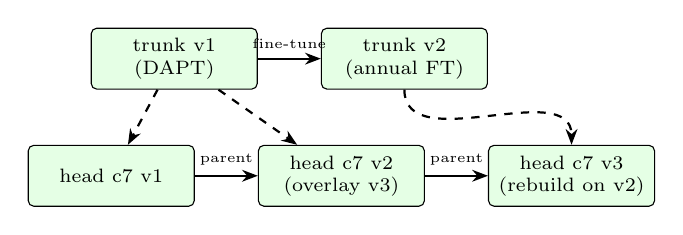
\begin{tikzpicture}[node distance=4mm and 8mm]
\node[model] (t1) {trunk v1\\(DAPT)};
\node[model, right=of t1] (t2) {trunk v2\\(annual FT)};
\node[model, below=7mm of t1, xshift=-8mm] (h11) {head c7 v1};
\node[model, right=of h11] (h12) {head c7 v2\\(overlay v3)};
\node[model, right=of h12] (h21) {head c7 v3\\(rebuild on v2)};
\draw[arr] (t1) -- node[lbl, above] {fine-tune} (t2);
\draw[darr] (t1) -- (h11);
\draw[darr] (t1) -- (h12);
\draw[darr] (t2.south) to[out=-90,in=90] (h21.north);
\draw[arr] (h11) -- node[lbl, above] {parent} (h12);
\draw[arr] (h12) -- node[lbl, above] {parent} (h21);
\end{tikzpicture}%
}
\caption{Lineage DAG. Solid edges: parent (fine-tune/warm-start). Dashed: trunk dependency. Every node carries its dataset, label-set, and overlay versions.}
\label{fig:dag}
\end{figure}

\section{Orchestrated Cadence}
Fig.~\ref{fig:cadence} shows the two loops from the companion system~[1], expressed as managed jobs.

\textbf{Monthly (head refresh).} Materialize the month's incremental recipe; append-embed new records; apply current label rules and overlays; retrain all heads; recalibrate thresholds; run the regression gate (each head's metrics vs.\ its prior version); commit a new manifest. Every step writes rows; the whole month is one auditable job chain.

\textbf{Annual (trunk refresh).} Fine-tune or re-DAPT the trunk on the grown corpus (recorded as a job with \texttt{parent\_model\_id}); re-embed the full corpus; rebuild all heads; atomic manifest cutover. On-demand jobs (a requirement change in C, a batch of adjudications) run the same machinery on one head.

Rollback at any cadence is a manifest revert: artifacts are immutable, versions only accumulate.

\begin{figure}[t]
\centering
\resizebox{\columnwidth}{!}{%
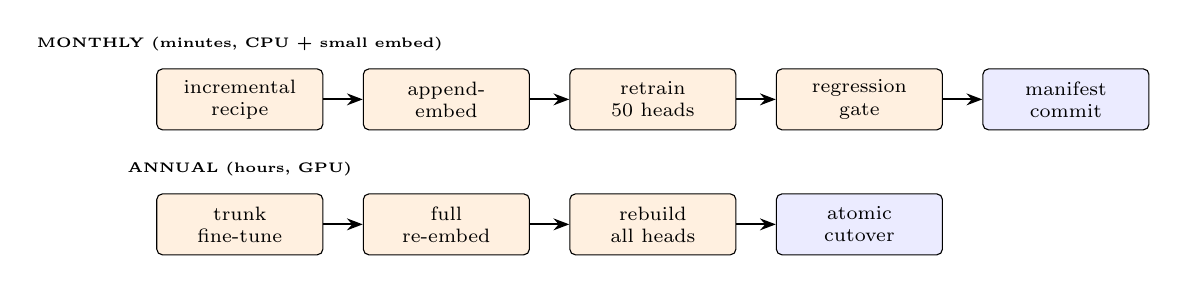
\begin{tikzpicture}[node distance=3.5mm and 5mm]
\node[process] (m1) {incremental\\recipe};
\node[process, right=of m1] (m2) {append-\\embed};
\node[process, right=of m2] (m3) {retrain\\50 heads};
\node[process, right=of m3] (m4) {regression\\gate};
\node[artifact, right=of m4] (m5) {manifest\\commit};
\node[above=1mm of m1, font=\tiny\bfseries] {MONTHLY (minutes, CPU + small embed)};
\node[process, below=8mm of m1] (a1) {trunk\\fine-tune};
\node[process, right=of a1] (a2) {full\\re-embed};
\node[process, right=of a2] (a3) {rebuild\\all heads};
\node[artifact, right=of a3] (a4) {atomic\\cutover};
\node[above=1mm of a1, font=\tiny\bfseries] {ANNUAL (hours, GPU)};
\draw[arr] (m1) -- (m2); \draw[arr] (m2) -- (m3); \draw[arr] (m3) -- (m4); \draw[arr] (m4) -- (m5);
\draw[arr] (a1) -- (a2); \draw[arr] (a2) -- (a3); \draw[arr] (a3) -- (a4);
\end{tikzpicture}%
}
\caption{Cadence as managed job chains. Monthly holds minimum viable product; annual refreshes the representation.}
\label{fig:cadence}
\end{figure}

\section{Reproducibility Guarantees}
For any registered model: (1)~its dataset is reconstructable by recipe re-execution against the recorded snapshot; (2)~its labels are reconstructable from the label rule version plus overlay version; (3)~its training is re-runnable from recorded hyperparameters and parent model; (4)~its deployment history is the git log of the manifest. The guarantee is structural---enforced by foreign keys and immutable artifacts---not procedural.

\section{Discussion}
The architecture's generality follows from its abstractions: typed sources, recipes, rules, overlays, and a lineage DAG describe any supervised program whose labels derive from an authoritative repository and whose corrections come from humans. The companion classifier~[1] is its first tenant; subsequent model programs join by adding rows, not systems.

\begin{thebibliography}{1}
\bibitem{mh} J.~Morgan, ``A Frozen-Trunk Multi-Head Architecture for Citation-Fidelity Remediation via Positive-Unlabeled Learning,'' companion paper, 2026.
\end{thebibliography}

\end{document}
